\section{RX Output}

The RX Output module takes packets from the main RX FIFO and sends
them out via the host interface, temporarially storing them in an
internal FIFO.

To read the packet out of the RX FIFO in its entierty into a buffer,
and then transmit, would incur a very long (~10 us) delay, hurting
latency. Instead, at our peril, we just begin transmitting the packets
out of the memory into an async fifo.

Note that the timing here is tricky. While its true that the memory
interface operates at 62.5 MHz per 16-bit-word, and this should be
strictly faster than the output interface (which is constrained to be
< 60) various delays in the system may result in DOUTEN not being high
for the entire duration of the packet.

The assertion of \signal{NEXTFRAME} by the host means "I am ready for
an inbound frame.'' Once \signal{NEXTFRAME} is asserted, it should not
be deasserted until \signal{DOEN} has gone high.


\subsection{Implementation}
The FSM checks every CLKEN period for the base pointer input to differ
from the stored BP value. We wait for, and synchronize with CLKEN to
make sure that we can correctly account for the RX FIFO interface read
latency.


We then latch the length and begin adding the packets to the output
FIFO. Should the output FIFO become full, the FSM transitions to the
\state{FIFONOP} state and waits until the FIFO is less than half-full
(signal \signal{HALFULL = 0}.

We verify the RX FIFO CRC with a CRC Verify module, and assert
\signal{MEMCRCERR} if there is an error. The memory CRC is sent out
via the output as well. 

\begin{figure}
\label{rxoutput}
\includegraphics[scale=0.7]{rxoutput.svg}
\caption{The RX Input, verifying correct packets}
\end{figure}

\begin{figure}
\label{rxoutputfsm}
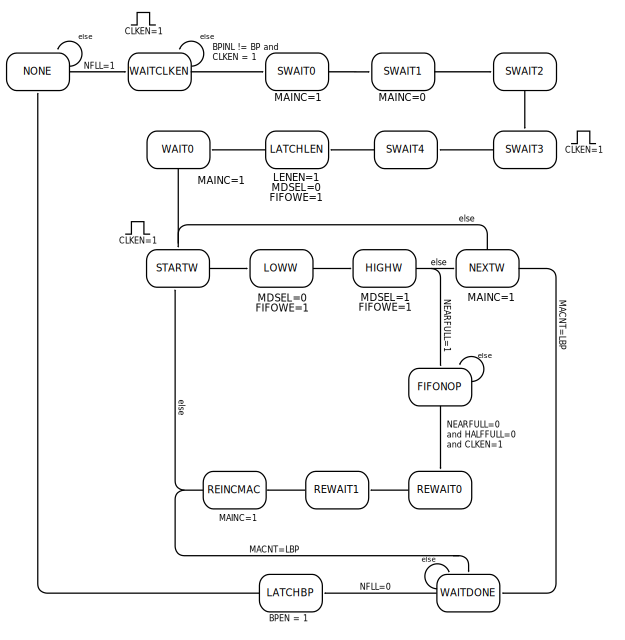
\includegraphics[scale=0.7]{rxoutput.fsm.svg}
\caption{The RX Input FSM, verifying correct packets}
\end{figure}

